\chapter{Hebrews 4}

\begin{figure}
  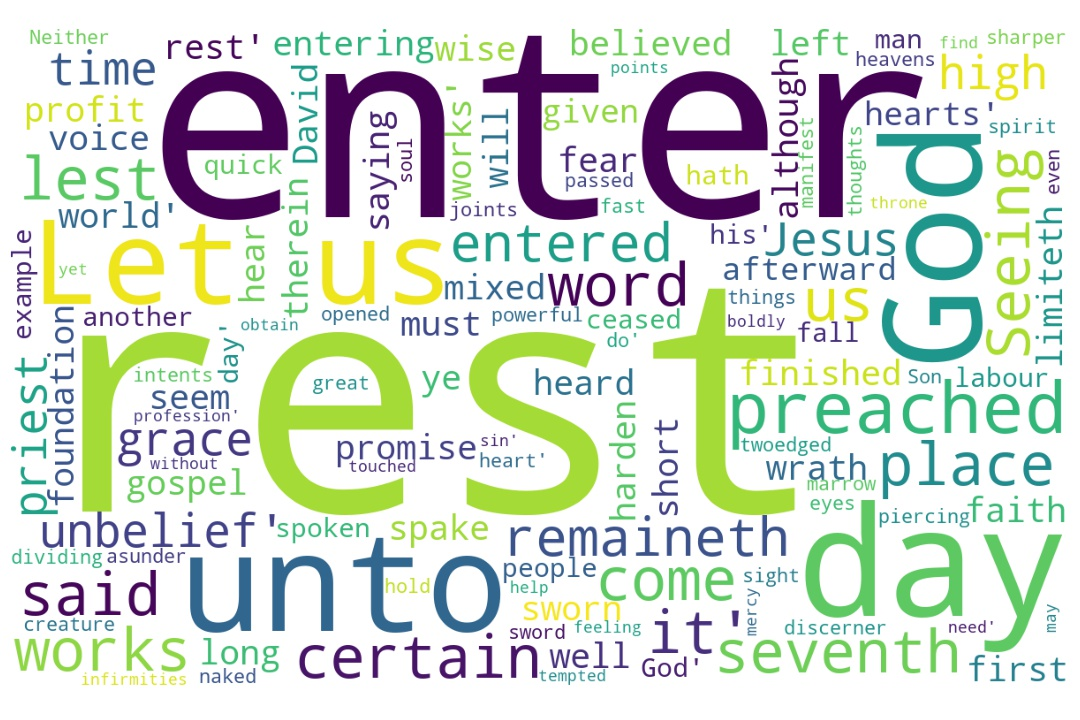
\includegraphics[width=\linewidth]{58NT-Hebrews/Hebrews4-WordCloud.jpg}
  \caption{Hebrews 4 Word Cloud}
  \label{fig:Hebrews 4 Word Cloud}
\end{figure}


\marginpar{\scriptsize \centering \fcolorbox{bone}{lime}{\textbf{A PATH TO REST}}\\ (Hebrews 4:1-16) \begin{compactenum}[I.][8]
    \item Coming \textbf{Short} \index[scripture]{Hebrews!Heb 04:01} (Hebrews 4:1)
    \item Wrath \textbf{Sworn} by God \index[scripture]{Hebrews!Heb 04:03} (Hebrews 4:3)
    \item \textbf{Shown} in Creation \index[scripture]{Hebrews!Heb 04:04} (Hebrews 4:4)
    \item \textbf{Spoken} by David \index[scripture]{Hebrews!Heb 04:07} (Hebrews 4:7) (see Psalm 95)
    \item \textbf{Ceasing} from Works \index[scripture]{Hebrews!Heb 04:10} (Hebrews 4:10)
    \item \textbf{Seeing} the Great High Priest \index[scripture]{Hebrews!Heb 04:14} (Hebrews 4:14)
    \item \textbf{Seeking} Mercy \index[scripture]{Hebrews!Heb 04:16} (Hebrews 4:16)\end{compactenum}}

\marginpar{\scriptsize \centering \fcolorbox{bone}{yellow}{\textbf{AVAILABLE}}\\ (Hebrews 4:1-16) \begin{compactenum}[I.][8]
    \item The \textbf{Promise} \index[scripture]{Hebrews!Heb 04:01} (Hebrews 4:1)
    \item The \textbf{Profit} \index[scripture]{Hebrews!Heb 04:02} (Hebrews 4:2)
    \item The \textbf{Preaching} \index[scripture]{Hebrews!Heb 04:02} (Hebrews 4:2, 6) \index[scripture]{Hebrews!Heb 04:06}
    \item The \textbf{Piercing} \index[scripture]{Hebrews!Heb 04:12} (Hebrews 4:12)
    \item The \textbf{Profit} \index[scripture]{Hebrews!Heb 04:14} (Hebrews 4:14)
\end{compactenum}}
    
% \textcolor[cmyk]{0.99998,1,0,0}{
% \footnote{\textcolor[cmyk]{0.99998,1,0,0}{\hyperlink{TOC}{Return to end of Table of Contents.}}}\footnote{\href{https://www.audioverse.org/english/audiobibles/books/ENGKJV/N/Heb/1}{\textcolor[cmyk]{0.99998,1,0,0}{Hebrews Audio}}}

\footnote{\textcolor[cmyk]{0.99998,1,0,0}{\hyperlink{TOC}{Return to end of Table of Contents.}}}\footnote{\href{https://www.audioverse.org/english/audiobibles/books/ENGKJV/N/Heb/1}{\textcolor[cmyk]{0.99998,1,0,0}{Hebrews Audio}}}\textcolor[cmyk]{0.99998,1,0,0}{Let us therefore fear, lest, a promise being left \emph{us} of entering into his rest, any of you should seem to \fcolorbox{bone}{lime}{come short} of it.}
[2] \textcolor[cmyk]{0.99998,1,0,0}{For unto us was the gospel preached, as well as unto them: but the word preached did not profit them, not being mixed with faith in them that heard \emph{it}.}
[3] \textcolor[cmyk]{0.99998,1,0,0}{For we which have believed do enter into rest, as he said, As I have \fcolorbox{bone}{lime}{sworn in my wrath}, if they shall enter into my rest: although the works were finished from the foundation of the world.}\footnote{\textbf{Psalm 95:11} - Unto whom I sware in my wrath that they should not enter into my rest.} 
[4] \textcolor[cmyk]{0.99998,1,0,0}{For he spake in a certain place of the seventh \emph{day} on this wise, And \fcolorbox{bone}{lime}{God did rest the seventh} \fcolorbox{bone}{lime}{day} from all his works.}\footnote{\textbf{Genesis 2:2} - And on the seventh day God ended his work which he had made; and he rested on the seventh day from all his work which he had made.}\footnote{\textbf{Exodus 20:11} - For in six days the LORD made heaven and earth, the sea, and all that in them is, and rested the seventh day: wherefore the LORD blessed the sabbath day, and hallowed it.}\footnote{\textbf{Exodus 31:17} - It is a sign between me and the children of Israel for ever: for in six days the LORD made heaven and earth, and on the seventh day he rested, and was refreshed.} 
[5] \textcolor[cmyk]{0.99998,1,0,0}{And in this \emph{place} again, If they shall enter into my rest.}
[6] \textcolor[cmyk]{0.99998,1,0,0}{Seeing therefore it remaineth that some must enter therein, and they to whom it was first preached entered not in because of unbelief:}
[7] \textcolor[cmyk]{0.99998,1,0,0}{Again, he limiteth a certain day, \fcolorbox{bone}{lime}{saying in David}, To day, after so long a time; as it is said, To day if ye will hear his voice, harden not your hearts.}\footnote{\textbf{Psalm 95:7} - For he is our God; and we are the people of his pasture, and the sheep of his hand. To day if ye will hear his voice,}
[8] \textcolor[cmyk]{0.99998,1,0,0}{For if Jesus had given them rest, then would he not afterward have spoken of another day.}
[9] \textcolor[cmyk]{0.99998,1,0,0}{There remaineth therefore a rest to the people of God.}\footnote{\textbf{Isaiah 11:10} - And in that day there shall be a root of Jesse, which shall stand for an ensign of the people; to it shall the Gentiles seek: and his rest shall be glorious.}\footnote{\textbf{Ezekiel 34:14} - I will feed them in a good pasture, and upon the high mountains of Israel shall their fold be: there shall they lie in a good fold, and in a fat pasture shall they feed upon the mountains of Israel.}\footnote{\textbf{Zephaniah 3:17} - The LORD thy God in the midst of thee is mighty; he will save, he will rejoice over thee with joy; he will rest in his love, he will joy over thee with singing.} 
[10] \textcolor[cmyk]{0.99998,1,0,0}{For he that is entered into his rest, he also hath \fcolorbox{bone}{lime}{ceased} from his own works, as God \emph{did} from his.}
[11] \textcolor[cmyk]{0.99998,1,0,0}{Let us labour therefore to enter into that rest, lest any man fall after the same example of unbelief.}
[12] \textcolor[cmyk]{0.99998,1,0,0}{For the word of God \emph{is} quick, and powerful, and sharper than any twoedged sword, piercing even to the dividing asunder of soul and spirit, and of the joints and marrow, and \emph{is} a discerner of the thoughts and intents of the heart.}\marginpar{\scriptsize \textcolor[rgb]{0.00,0.545,0.269}{$\rightarrow$ The word of God:
\begin{compactenum}[1.]
	\item is quick (living)
	\item powerful
	\item sharper than any twoedged sword
	\item divides soul \& spirit
	\item discerns the thoughts and intents of the heart
	\item Is given the attributes of God in verse 13 (his), namely, onmiscience
\end{compactenum}}    }
[13] \textcolor[cmyk]{0.99998,1,0,0}{Neither is there any creature that is not manifest in his sight: but all things \emph{are} naked and opened unto the eyes of him with whom we have to do.}
[14] \textcolor[cmyk]{0.99998,1,0,0}{Seeing then that we have a \fcolorbox{bone}{lime}{great high priest}, that is passed into the heavens, Jesus the Son of God, let us hold fast \emph{our} profession.}
[15] \textcolor[cmyk]{0.99998,1,0,0}{For we have not an high priest which cannot be touched with the feeling of our infirmities; but was in all points tempted like as \emph{we} \emph{are,} \emph{yet} without sin.}
[16] \textcolor[cmyk]{0.99998,1,0,0}{Let us therefore come boldly unto the throne of grace, that we may \fcolorbox{bone}{lime}{obtain mercy}, and find grace to help in time of need.}
